
\begin{figure}[H]
\centering
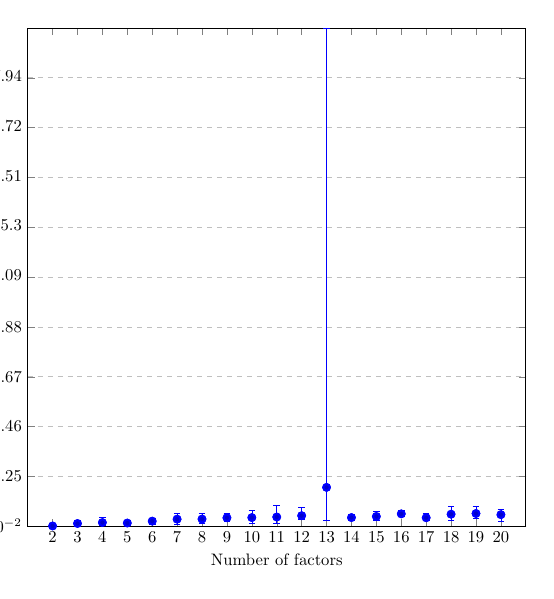
\begin{tikzpicture}[scale=0.6, trim axis left, trim axis right]
\begin{axis}[
    width=1\textwidth,
    height=1\textwidth,
    xlabel={Number of factors},
    ylabel={Time taken (s)},
    xmin=1.0, xmax=21.0,
    ymin=0.039878, ymax=2442.145914,
    xticklabels={2, 3, 4, 5, 6, 7, 8, 9, 10, 11, 12, 13, 14, 15, 16, 17, 18, 19, 20},
    xtick={2, 3, 4, 5, 6, 7, 8, 9, 10, 11, 12, 13, 14, 15, 16, 17, 18, 19, 20},
    ytick={0.039878, 244.2504816, 488.4610852, 732.6716888, 976.8822924, 1221.092896, 1465.3034996, 1709.5141032, 1953.7247068, 2197.9353104},
    ymajorgrids=true,
    grid style=dashed,
]

\addplot+[
    blue,
    very thick,
    forget plot,
    only marks
    ]
    plot[
    very thick,
    error bars/.cd,
    y dir=plus,
    y explicit
    ]
    table[x=x,y=y,y error expr=\thisrow{y-max}] {
    x    y    y-max
    11	44.79045125	56.38082775
10	41.9667662	33.6286648
13	189.979366118	2252.16654788
12	51.3558824	40.9458316
15	47.6032968	25.9382302
14	42.0610622	17.5830458
17	41.0848572	22.9701568
16	60.2416763	16.2652167
19	62.138151	33.673764
18	58.5388423	38.6376287
20	56.2998739	25.4871101
3	13.0466173714	17.7063666286
2	0.9197989	1.1922671
5	15.2649996	14.0374764
4	17.68552625	26.76513775
7	34.28858725	26.88017075
6	24.56607165	12.86654935
9	41.11818965	19.68379035
8	34.69769485	26.94538015

    };

\addplot+[
    blue,
    very thick,
    forget plot,
    only marks
    ]
    plot[
    very thick,
    error bars/.cd,
    y dir=plus,
    y explicit
    ]
    table[x=x,y=y,y error expr=\thisrow{y-min}] {
    x    y    y-min
    11	44.79045125	-32.18917725
10	41.9667662	-27.0611902
13	189.979366118	-163.265396118
12	51.3558824	-20.3187674
15	47.6032968	-17.7107468
14	42.0610622	-14.7735332
17	41.0848572	-13.6113412
16	60.2416763	-13.1950613
19	62.138151	-21.511895
18	58.5388423	-29.0222243
20	56.2998739	-31.7420959
3	13.0466173714	-11.9691843714
2	0.9197989	-0.8799209
5	15.2649996	-9.1448556
4	17.68552625	-15.67773625
7	34.28858725	-23.91962725
6	24.56607165	-14.42937465
9	41.11818965	-15.21486565
8	34.69769485	-19.83394085

    };

\end{axis}
\end{tikzpicture}
\vspace{-0.3cm}
\caption{Larger primes}\label{fig:LenstrasEllipticCurveFactorizationLargerprimes(maximumIterations:-1)factors}
\end{figure}
